\chapter{Общие сведения теории формальных языков}\label{chpt:FormalLanguageTheoryIntro}

В данной главе мы рассмотрим основные понятия из теории формальных языков, которые пригодятся нам в дальнейшем изложении.

\begin{definition}
\textit{Алфавит} --- это конечное множество.
Элементы этого множества будем называть \textit{символами}.
\end{definition}

\begin{example}
  Примеры алфавитов

  \begin{itemize}
    \item Латинский алфавит $\Sigma = \{ a, b, c, \dots, z\}$
    \item Кириллический алфавит $\Sigma = \{ \text{а, б, в, \dots, я}\}$
    \item Алфавит чисел в шестнадцатеричной записи 
    $$\Sigma = \{0, 1, 2, 3, 4, 5, 6, 7 ,8,9, A, B, C, D, E, F \}$$
  \end{itemize}
\end{example}

Традиционное обозначение для алфавита --- $\Sigma$.
Также мы будем использовать различные прописные буквы латинского алфавита. Для обозначения символов алфавита будем использовать строчные буквы латинского алфавита: $a, b, \dots, x, y, z$.

Будем считать, что над алфавитом $\Sigma$ всегда определена операция конкатенации $(\cdot): \Sigma^* \times \Sigma^* \to \Sigma^*$.
При записи выражений символ точки (обозначение операции конкатенации) часто будем опускать: $a \cdot b = ab$.

\begin{definition}
\textit{Слово} над алфавитом $\Sigma$ --- это конечная конкатенация символов алфавита $\Sigma$: $\omega = a_0 \cdot a_1 \cdot \ldots \cdot a_m$, где $\omega$ --- слово, а для любого $i$ $a_i \in \Sigma$.
\end{definition}

\begin{definition}
Пусть $\omega = a_0 \cdot a_1 \cdot \ldots \cdot a_m$ --- слово над алфавитом $\Sigma$.
Будем называть $m + 1$ \textit{длиной слова} и обозначать как $|\omega|$.
\end{definition}

\begin{definition}
\textit{Язык} над алфавитом $\Sigma$ --- это множество слов над алфавитом $\Sigma$.
\end{definition}

\begin{example}

Примеры языков.

  \begin{itemize}
    \item Язык целых чисел в двоичной записи $\{0, 1, -1, 10, 11, -10, -11, \dots\}.$
    \item Язык всех правильных скобочных последовательностей $$\{(), (()), ()(), (())(), \dots\}.$$
  \end{itemize}
\end{example}

Любой язык над алфавитом $\Sigma$ является подмножеством $\Sigma^*$ --- множества всех слов над алфавитом $\Sigma$.

Заметим, что язык не обязан быть конечным множеством, в то время как алфавит всегда конечен и изучаем мы конечные слова.

%\begin{definition}
\textit{Способы задания языков}
\begin{itemize}
\item Перечислить все элементы. Такой способ работает только для конечных языков. Перечислить бесконечное множество не получится.
\item Задать генератор --- процедуру, которая возвращает очередное слово языка.
\item Задать распознователь --- процедуру, которая по данному слову может определить, принадлежит оно заданному языку или нет.
\end{itemize}


\section{Контекстно-свободные грамматики и языки}\label{CFG}

Из всего многообразия нас будут интересовать прежде всего контекстно-свободные грамматики.

\begin{definition}
\textit{Контекстно-свободная грамматика} --- это четвёрка вида $\langle \Sigma, N, P, S \rangle$, где
\begin{itemize}
  \item $\Sigma$ --- это терминальный алфавит;
  \item $N$ --- это нетерминальный алфавит;
  \item $P$ --- это множество правил или продукций, таких что каждая продукция имеет вид $N_i \to \alpha$, где $N_i \in N$ и $\alpha \in \{\Sigma \cup N\}^* \cup {\varepsilon}$;
  \item $S$ --- стартовый нетерминал.
  Отметим, что $\Sigma \cap N = \varnothing$.
\end{itemize}
\end{definition}

\begin{example}
Грамматика, задающая язык целых чисел в двоичной записи без лидирующих нулей: $G = \langle \{0, 1, -\}, \{S, N, A\}, P, S \rangle$, где $P$ определено следующим образом:

\[
\begin{array}{rcl}
S& \rightarrow & 0 \mid N \mid - N  \\
N& \rightarrow & 1 A \\
A& \rightarrow & 0 A \mid 1 A  \mid \varepsilon\\
\end{array}
\]
\end{example}

При спецификации грамматики часто опускают множество терминалов и нетерминалов, оставляя только множество правил. При этом нетерминалы часто обозначаются прописными латинскими буквами, терминалы --- строчными, а стартовый нетерминал обозначается буквой~$S$. Мы будем следовать этим обозначениям, если не указано иное.


\begin{definition}\label{def derivability in CFG}
  \textit{Отношение непосредственной выводимости}. Мы говорим, что последовательность терминалов и нетерминалов $\gamma \alpha \delta$ \textit{непосредственно выводится из} $\gamma \beta \delta$ \textit{при помощи правила} $\alpha \rightarrow \beta$ ($\gamma \alpha \delta \Rightarrow \gamma \beta \delta$), если
  \begin{itemize}
    \item $\alpha \rightarrow \beta \in P$
    \item $\gamma, \delta \in \{\Sigma \cup N\}^* \cup {\varepsilon}$
  \end{itemize}
\end{definition}

\begin{definition}
  \textit{Рефлексивно-транзитивное замыкание отношения} --- это наименьшее рефлексивное и транзитивное отношение, содержащее исходное.
\end{definition}

\begin{definition}
\textit{Отношение выводимости} является рефлексивно-транзитивным замыканием отношения непосредственной выводимости
\begin{itemize}
  \item $\alpha \derives \beta$ означает $\exists \gamma_0, \dots \gamma_k: \ \alpha \derives[] \gamma_0 \derives[] \gamma_1 \derives[] \dots \derives[] \gamma_{k-1} \derives[] \gamma_{k} \derives[] \beta$
  \item Транзитивность: $\forall \alpha, \beta, \gamma \in \{\Sigma \cup N\}^* \cup {\varepsilon}: \ \alpha \derives \beta, \beta \derives \gamma \Rightarrow \alpha \derives \gamma$
  \item Рефлексивность: $\forall \alpha \in \{\Sigma \cup N\}^* \cup {\varepsilon}: \ \alpha \derives \alpha$
  \item $\alpha \derives \beta$ --- $\alpha$ выводится из $\beta$
  \item $\alpha \derives[k] \beta$ --- $\alpha$ выводится из $\beta$ за $k$ шагов
  \item $\alpha \derives[+] \beta$ --- при выводе использовалось хотя бы одно правило грамматики
\end{itemize}
\end{definition}


\begin{example}
Пример вывода цепочки $-1101$ в грамматике:

  \[
  \begin{array}{rcl}
  S& \rightarrow & 0 \mid N \mid - N  \\
  N& \rightarrow & 1 A \\
  A& \rightarrow & 0 A \mid 1 A  \mid \varepsilon\\
  \end{array}
  \]

  \[ S \Rightarrow - N \Rightarrow - 1 A \Rightarrow - 1 1 A \derives - 1 1 0 1 A \Rightarrow - 1 1 0 1 \]
\end{example}


\begin{definition}[Вывод слова в грамматике]
Слово $\omega \in \Sigma^*$ \textit{выводимо в грамматике} $\langle \Sigma, N, P, S \rangle$, если существует некоторый вывод этого слова из начального нетерминала $S \derives \omega$.

\end{definition}

\begin{definition}
\textit{Левосторонний вывод}. На каждом шаге вывода заменяется самый левый нетерминал.
\end{definition}

\begin{example}
Пример левостороннего вывода цепочки в грамматике

  \[
    \begin{array}{rcl}
    S& \rightarrow & A A \mid s  \\
    A& \rightarrow & A A \mid B b \mid a \\
    B& \rightarrow & c \mid d
    \end{array}
  \]

  \[ \boldsymbol{S} \derives[] \boldsymbol{A} A \derives[] \boldsymbol{B} b A \derives[] c b \boldsymbol{A} \derives[] c b \boldsymbol{A} A \derives[] c b a \boldsymbol{A} \derives[] c b a a \]
\end{example}

Аналогично можно определить правосторонний вывод.

\begin{definition}
\textit{Язык, задаваемый грамматикой} --- множество строк, выводимых в грамматике $L(G) = \{ \omega \in \Sigma^* \mid S \derives \omega \}$.
\end{definition}

\begin{definition}
  Грамматики $G_1$ и $G_2$ называются \textit{эквивалентными}, если они задают один и тот же язык: $L(G_1) = L(G_2)$
\end{definition}


\begin{example}  Пример эквивалентных грамматик для языка целых чисел в двоичной системе счисления.

  \begin{tabular}{p{0.4\textwidth} | p{0.5\textwidth}}

    \[
      \begin{array}{rcl}
      \Sigma &=& \{ 0, 1, - \} \\
      N &=& \{ S, N, A \} \\~\\
      S& \rightarrow & 0 \mid N \mid - N  \\
      N& \rightarrow & 1 A \\
      A& \rightarrow & 0 A \mid 1 A  \mid \varepsilon\\
      \end{array}
    \]

    &

    \[
      \begin{array}{rcl}
      \Sigma &=& \{ 0, 1, - \} \\
      N &=& \{ S, A \} \\~\\
      S& \rightarrow & 0 \mid 1 A  \mid - 1 A  \\
      A& \rightarrow &  0 A \mid 1 A  \mid \varepsilon\\
      \end{array}
    \]
    \end{tabular}

\end{example}


\begin{definition}
  \textit{Неоднозначная грамматика} --- грамматика, в которой существует 2 и более левосторонних (правосторонних) выводов для одного слова.
\end{definition}

\begin{example}
  Неоднозначная грамматика для правильных скобочных последовательностей

\[
    S \to (S) \mid S S \mid \varepsilon
\]
\end{example}

\begin{definition}
  \textit{Однозначная грамматика} --- грамматика, в которой существует не более одного левостороннего (правостороннего) вывода для каждого слова.
\end{definition}

\begin{example}
  Однозначная грамматика для правильных скобочных последовательностей

\[
    S \to (S)S \mid \varepsilon
\]
\end{example}

\begin{definition}
  \textit{Существенно неоднозначные языки} --- языки, для которых невозможно построить однозначную грамматику.
\end{definition}

\begin{example}
  Пример существенно неоднозначного языка

\[\{a^n b^n c^m \mid n, m \in \mathds{Z}\} \cup \{a^n b^m c^m \mid n,m \in \mathds{Z}\}\]
\end{example}

\section{Дерево вывода}\label{sect:DerivTree}
В некоторых случаях не достаточно знать порядок применения правил.
Необходимо структурное представление вывода цепочки в грамматике.
Таким представлением является \textit{дерево вывода}.
\begin{definition}
Деревом вывода цепочки $\omega$ в грамматике $G=\langle \Sigma, N, S, P \rangle$ называется дерево, удовлетворяющее следующим свойствам.

\begin{enumerate}
  \item Помеченное: метка каждого внутреннего узла --- нетерминал, метка каждого листа --- терминал или $\varepsilon$.
  \item Корневое: корень помечен стартовым нетерминалом.
  \item Упорядоченное.
  \item В дереве может существовать узел с меткой $N_i$ и сыновьями $M_j \dots M_k$ только тогда, когда в грамматике есть правило вида $N_i \to M_j \dots M_k$.
  \item Крона образует исходную цепочку $\omega$.
\end{enumerate}
\end{definition}

\begin{example}
  Построим дерево вывода цепочки $ababab$ в грамматике

  \[ G = \langle \{a,b\}, \{S\}, S, \{S \to a \ S \ b \ S, S \to \varepsilon\} \rangle \]

\begin{center}

    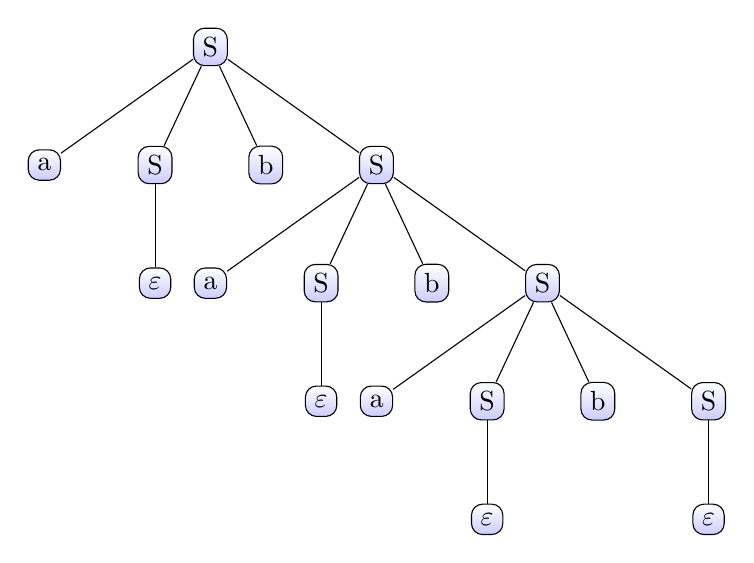
\begin{tikzpicture}[sibling distance=4em,
    every node/.style = {shape=rectangle, rounded corners,
      draw, align=center,
      top color=white, bottom color=blue!20}]]
    \node {S}
      child { node {a} }
      child { node {S}
        child { node {$\varepsilon$}}
      }
      child { node {b} }
      child { node {S}
        child {node {a}}
        child { node {S}
          child { node {$\varepsilon$}}
        }
        child { node {b} }
        child { node {S}
          child {node {a}}
          child {node {S}
            child {node {$\varepsilon$}}
          }
          child {node {b}}
          child {node {S}
            child {node {$\varepsilon$}}
          }
        }
      };
  \end{tikzpicture}
\end{center}

\end{example}

\begin{theorem}
  Пусть $G = \langle \Sigma, N, P, S \rangle$ --- КС-грамматика.
  Вывод $S \derives \alpha$, где $\alpha \in (N \cup \Sigma)^*, \alpha \neq \varepsilon$ существует $\Leftrightarrow$ существует дерево вывода в грамматике $G$ с кроной $\alpha$.
\end{theorem}

\section{Пустота КС-языка}

\begin{theorem}
  Существует алгоритм, определяющий, является ли язык, порождаемый КС грамматикой, пустым.
\end{theorem}

\begin{proof}
  Следующая лемма утверждает, что если в КС языке есть выводимое слово, то существует другое выводимое слово с деревом вывода не глубже количества нетерминалов грамматики.
  Для доказательства теоремы достаточно привести алгоритм, последовательно строящий все деревья глубины не больше количества нетерминалов грамматики, и проверяющий, являются ли такие деревья деревьями вывода.
  Если в результате работы алгоритма не удалось построить ни одного дерева, то грамматика порождает пустой язык.
\end{proof}

\begin{lemma}
  Если в данной грамматике выводится некоторая цепочка, то существует цепочка, дерево вывода которой не содержит ветвей длиннее m, где m --- количество нетерминалов грамматики.
\end{lemma}

\begin{proof}
  Рассмотрим дерево вывода цепочки $\omega$. Если в нем есть 2 узла, соответствующих одному нетерминалу A, обозначим их $n_1$ и $n_2$.

  Предположим, $n_1$ расположен ближе к корню дерева, чем $n_2$.

  $S \derives \alpha A_{n_1} \beta \derives \alpha \omega_1 \beta; S \derives \alpha \gamma A_{n_2} \delta \beta \derives \alpha \gamma \omega_2 \delta \beta$, при этом $\omega_2$ является подцепочкой $\omega_1$.

  Заменим в изначальном дереве узел $n_1$ на $n_2$. Полученное дерево является деревом вывода $\alpha \omega_2 \delta$.

  Повторяем процесс замены одинаковых нетерминалов до тех пор, пока в дереве не останутся только уникальные нетерминалы.

  В полученном дереве не может быть ветвей длины большей, чем m.

  По построению оно является деревом вывода.
\end{proof}


\section{Нормальная форма Хомского}
\label{section:CNF}

\begin{definition}
Контекстно-свободная грамматика $\langle \Sigma, N, P, S\rangle$ находится в \textit{Нормальной Форме Хомского}, если она содержит только правила следующего вида:

\begin{itemize}
  \item $A \to B C \text{, где } A, B, C \in N \text{, S не содержится в правой части правила }$
  \item $A \to a \text{, где } A \in N, a \in \Sigma$
  \item $S \to \varepsilon$
\end{itemize}
\end{definition}

\begin{theorem}
Любую КС грамматику можно преобразовать в НФХ.
\end{theorem}

\begin{proof}
  Алгоритм преобразования в НФХ состоит из следующих шагов:

  \begin{itemize}
    \item Замена неодиночных терминалов
    \item Удаление длинных правил
    \item Удаление $\varepsilon$-правил
    \item Удаление цепных правил
    \item Удаление бесполезных нетерминалов
  \end{itemize}

  То, что каждый из этих шагов преобразует грамматику к эквивалентной, при этом является алгоритмом, доказано в следующих леммах.
\end{proof}

\begin{lemma}
  Для любой КС-грамматики можно построить эквивалентную, которая не содержит правила с неодиночными терминалами.
\end{lemma}

\begin{proof}
  Каждое правило $A \to B_0 B_1 \dots B_k, k \geq 1$ заменить на множество правил:
  \begin{itemize}
    \item $A \to C_0 C_1 \dots C_k$
    \item $\{ C_i \to B_i \mid B_i \in \Sigma, C_i \text{ --- новый нетерминал} \}$
  \end{itemize}
\end{proof}

\begin{lemma}
  Для любой КС-грамматики можно построить эквивалентную, которая не содержит правил длины больше 2.
\end{lemma}

\begin{proof}
  Каждое правило $A \to B_0 B_1 \dots B_k, k \geq 2$ заменить на множество правил:
  \begin{itemize}
    \item $A \to B_0 C_0$
    \item $C_0 \to B_1 C_1$
    \item $\dots$
    \item $C_{k-3} \to B_{k-2} C_{k-2}$
    \item $C_{k-2} \to B_{k-1} B_k$
  \end{itemize}
\end{proof}


\begin{lemma}
  Для любой КС-грамматики можно построить эквивалентную, не содержащую $\varepsilon$-правил.
\end{lemma}

\begin{proof}
  Определим $\varepsilon$-правила:
  \begin{itemize}
    \item $A \to \varepsilon$
    \item $A \to B_0 \dots B_k, \forall i: \ B_i$ --- $\varepsilon$-правило.
  \end{itemize}

  Каждое правило $A \to B_0 B_1 \dots B_k$ заменяем на множество правил, где каждое $\varepsilon$-правило удалено во всех возможных комбинациях.
\end{proof}

\begin{lemma}
  Можно удалить все цепные правила
\end{lemma}

\begin{proof}
  \textit{Цепное правило} --- правило вида $A \to B\text{, где } A, B \in N\\$.
  \textit{Цепная пара} --- упорядоченная пара $(A,B)$, в которой $A\derives B$, используя только цепные правила.
  
  Алгоритм:
  \begin{enumerate}
  \item Найти все цепные пары в грамматике $G$.
  Найти все цепные пары можно по индукции:
  Базис: $(A,A)$ --- цепная пара для любого нетерминала, так как $A\derives A$ за ноль шагов.
  Индукция: Если пара $(A,B_0)$ --- цепная, и есть правило $B_0 \to B_1$, то $(A,B_1)$ --- цепная пара.
  \item Для каждой цепной пары $(A,B)$ добавить в грамматику $G'$ все правила вида $A \to a$, где $B \to a$ --- нецепное правило из $G$.
  \item Удалить все цепные правила
\end{enumerate}
Пусть $G$ --- контекстно-свободная грамматика. $G'$ --- грамматика, полученная в результате применения алгоритма к $G$. Тогда $L(G)=L(G')$.
\end{proof}

\begin{definition}
Нетерминал $A$ называется \textit{порождающим}, если из него может быть выведена конечная терминальная цепочка. Иначе он называется \textit{непорождающим}.
\end{definition}

\begin{lemma}
  Можно удалить все бесполезные (непорождающие) нетерминалы
\end{lemma}

\begin{proof}
  После удаления из грамматики правил, содержащих непорождающие нетерминалы, язык не изменится, так как непорождающие нетерминалы по определению не могли участвовать в выводе какого-либо слова.
  
  Алгоритм нахождения порождающих нетерминалов:
  \begin{enumerate}
  \item Множество порождающих нетерминалов пустое.
  \item Найти правила, не содержащие нетерминалов в правых частях и добавить нетерминалы, встречающихся в левых частях таких правил, в множество.
  \item Если найдено такое правило, что все нетерминалы, стоящие в его правой части, уже входят в множество, то добавить в множество нетерминалы, стоящие в его левой части.
  \item Повторить предыдущий шаг, если множество порождающих нетерминалов изменилось.
\end{enumerate}
В результате получаем множество всех порождающих нетерминалов грамматики, а все нетерминалы, не попавшие в него, являются непорождающими. Их можно удалить.
\end{proof}

\begin{example}
  Приведем в Нормальную Форму Хомского однозначную грамматику правильных скобочных последовательностей: $S \to a S b S \mid \varepsilon$

  Первым шагом добавим новый нетерминал и сделаем его стартовым: 

  \begin{align*}
    S_0 &\to S  \\ 
    S   &\to a S b S \mid \varepsilon
  \end{align*}

  Заменим все терминалы на новые нетерминалы: 

  \begin{align*}
    S_0 &\to S \\ 
    S   &\to L S R S \mid \varepsilon \\ 
    L   &\to a \\ 
    R   &\to b
  \end{align*}

  Избавимся от длинных правил: 

  \begin{align*}
    S_0 &\to S \\ 
    S   &\to L S' \mid \varepsilon \\ 
    S'  &\to S S'' \\ 
    S'' &\to R S \\
    L   &\to a \\ 
    R   &\to b
  \end{align*}

  Избавимся от $\varepsilon$-продукций: 

  \begin{align*}
    S_0 &\to S \mid \varepsilon \\ 
    S   &\to L S' \\ 
    S'  &\to S'' \mid S S'' \\ 
    S'' &\to R   \mid R S \\
    L   &\to a \\ 
    R   &\to b
  \end{align*}

  Избавимся от цепных правил: 

  \begin{align*}
    S_0 &\to L S' \mid \varepsilon \\ 
    S   &\to L S' \\ 
    S'  &\to b \mid R S \mid S S'' \\ 
    S'' &\to b \mid R S \\
    L   &\to a \\ 
    R   &\to b
  \end{align*}
\end{example}

\begin{definition}\label{defn:wCNF}
Контекстно-свободная грамматика $\langle \Sigma, N, P, S\rangle$ находится в \textit{ослабленной Нормальной Форме Хомского}, если она содержит только правила следующего вида:

\begin{itemize}
  \item $A \to B C \text{, где } A, B, C \in N$
  \item $A \to a \text{, где } A \in N, a \in \Sigma$
  \item $A \to \varepsilon \text{, где } A \in N$
\end{itemize}

То есть ослабленная НФХ отличается от НФХ тем, что:
\begin{enumerate}
  \item $\varepsilon$ может выводиться из любого нетерминала
  \item $S$ может появляться в правых частях правил
\end{enumerate}
\end{definition}

\section{Лемма о накачке}

\begin{lemma}
Пусть $L$ --- контекстно-свободный язык над алфавитом $\Sigma$, тогда существует такое $n$, что для любого слова $\omega \in L$, $|\omega| \geq n$ найдутся слова $u,v,x,y,z\in \Sigma^*$, для которых верно: $uvxyz = \omega, vy\neq \varepsilon,|vxy|\leq n$ и для любого $k \geq 0$  $uv^kxy^kz \in L$.
\end{lemma}

Идея доказательства леммы о накачке.

\begin{enumerate}
    \item Для любого КС языка можно найти грамматику в нормальной форме Хомского.
    \item Очевидно, что если брать достаточно длинные цепочки, то в дереве вывода этих цепочек, на пути от корня к какому-то листу обязательно будет нетерминал, встречающийся минимум два раза. Если $m$ --- количество нетерминалов в НФХ, то длины $2^{m+1}$ должно хватить. Это и будет $n$ из леммы.
    \item Возьмём путь, на котором есть хотя бы дважды повторяется некоторый нетерминал. Скажем, это нетерминал  $N_1$. Пойдём от листа по этому пути. Найдём первое появление $N_1$. Цепочка, задаваемая поддеревом для этого узла --- это $x$ из леммы.
    \item Пойдём дальше и найдём второе появление $N_1$. Цепочка, задаваемая поддеревом для этого узла --- это $vxy$ из леммы.
    \item Теперь мы можем копировать кусок дерева между этими повторениями $N_1$ и таким образом накачивать исходную цепочку.
\end{enumerate}

Надо только проверить выполение ограничений на длины.

Нахождение разбиения и пример накачки продемонстрированы на рисунках~\ref{fig:pumping1} и~\ref{fig:pumping2}.

\begin{figure}
\centering
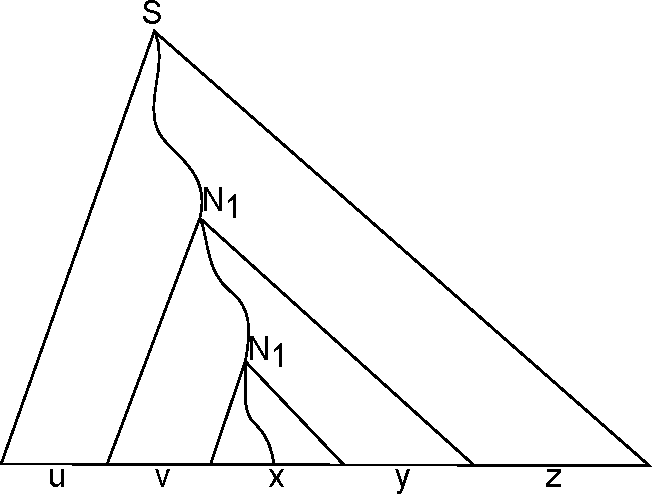
\includegraphics[width=0.5\textwidth]{pics/pumping_tree_1.pdf}
\caption{Разбиение цепочки для леммы о накачке}
\label{fig:pumping1}
\end{figure}

\begin{figure}
\centering
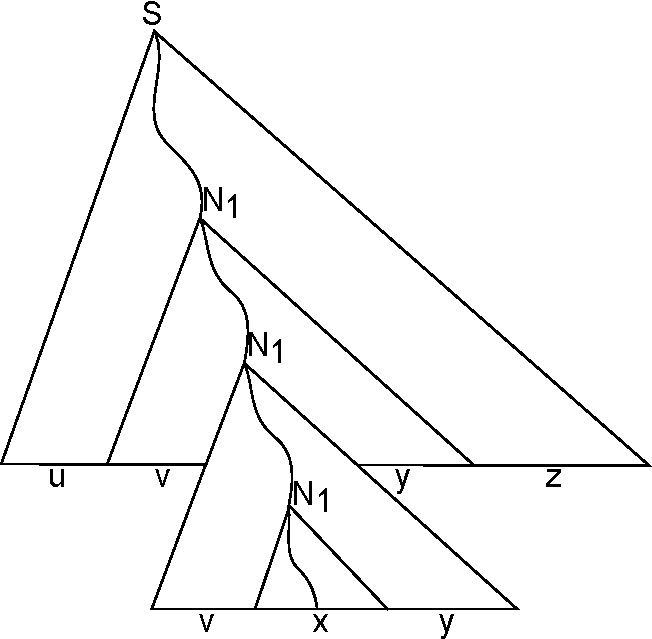
\includegraphics[width=0.5\textwidth]{pics/pumping_tree_2.pdf}
\caption{Пример накачки цепочки с рисунка~\ref{fig:pumping1}}
\label{fig:pumping2}
\end{figure}


Для примера предлагается проверить неконтекстно-свободность языка $L=\{a^nb^nc^n \mid n>0\}$.


\section{Замкнутость КС языков относительно операций}


\begin{theorem}
Контекстно-свободные языки замкнуты относительно следующих операций:
\begin{enumerate}
  \item Объединение: если $L_1$ и $L_2$ --- контекстно-свободные языки, то и $L_3 = L_1 \cup L_2$ --- контекстно-свободный.
  \item Конкатенация: если $L_1$ и $L_2$ --- контекстно-свободные языки, то и $L_3 = L_1 \cdot L_2$ --- контекстно-свободный.
  \item Замыкание Клини: если $L_1$ --- контекстно-свободный, то и $L_2 = \bigcup\limits_{i=0}^{\infty} L_1^i $ --- контекстно-свободный.
  \item Разворот: если $L_1$ --- контекстно-свободный, то и $L_2 = {L_1}^r$ --- контекстно-свободный.
  \item Пересечение с регулярными языками: если $L_1$ --- контекстно-свободный, а $L_2$ --- регулярный, то  $L_3 = L_1 \cap L_2$ --- контекстно-свободный.
  \item Разность с регулярными языками: если $L_1$ --- контекстно-свободный, а $L_2$ --- регулярный, то  $L_3 = L_1 \setminus L_2$ --- контекстно-свободный.
\end{enumerate}
\end{theorem}
Для доказательства пунктов 1--4 можно построить КС граммтику нового языка имея грамматики для исходных. 
Будем предполагать, что множества нетерминальных символов различных граммтик для исходных языков не пересекаются.
\begin{enumerate}
\item $G_1=\langle\Sigma_1,N_1,P_1,S_1\rangle$ --- граммтика для $L_1$, $G_1=\langle\Sigma_2,N_2,P_2,S_2\rangle$ --- граммтика для $L_2$, тогда $G_3=\langle\Sigma_1 \cup \Sigma_2, N_1 \cup N_2 \cup \{S_3\}, P_1 \cup P_2 \cup \{S_3 \to S_1 \mid S_2\} ,S_3\rangle$ --- граммтика для $L_3$. 

\item $G_1=\langle\Sigma_1,N_1,P_1,S_1\rangle$ --- граммтика для $L_1$, $G_1=\langle\Sigma_2,N_2,P_2,S_2\rangle$ --- граммтика для $L_2$, тогда $G_3=\langle\Sigma_1 \cup \Sigma_2, N_1 \cup N_2 \cup \{S_3\}, P_1 \cup P_2 \cup \{S_3 \to S_1 S_2\} ,S_3\rangle$ --- граммтика для $L_3$. 

\item $G_1=\langle\Sigma_1,N_1,P_1,S_1\rangle$ --- граммтика для $L_1$, тогда $G_2=\langle\Sigma_1, N_1 \cup \{S_2\}, P_1 \cup \{S_2 \to S_1 S_2\ \mid \varepsilon\}, S_2\rangle$ --- граммтика для $L_2$. 

\item $G_1=\langle\Sigma_1,N_1,P_1,S_1\rangle$ --- граммтика для $L_1$, тогда $G_2=\langle\Sigma_1, N_1, \{N^i \to \omega^R \mid N^i \to \omega \in P_1 \}, S_1\rangle$ --- граммтика для $L_2$. 
\end{enumerate}

Чтобы доказать замкнутость относительно пересечения с регулярными языками, построим по КС грамматике рекурсивный автомат $R_1$, по регулярному выражению --- детерминированный конечный автомат $R_2$, и построим их прямое произведение $R_3$.
Переходы по терминальным символам в новом автомате возможны тогда и только тогда, когда они возможны одновременно и в исходном рекурсивном автомате и в исходном конечном. 
За рекурсивные вызовы отвечает исходныа рекурсивный автомат. 
Значит цепочка принимается $R_3$ тогда и только тогда, когда она принимается одновременно $R_1$ и $R_2$: так как состояния $R_3$ --- это пары из состояния $R_1$ и $R_2$, то по трассе вычислений $R_3$ мы всегда можем построить трассу для $R_1$ и $R_2$ и наоборот.

Чтобы доказать замкнутость относительно разности с регулятным языком, достаточно вспомнить, что регулярные языки замкнуты относительно дополнения, и выразить разность через пересечение с дополнением: 
$$
L_1 \setminus L_2 = L_1 \cap \overline{L_2}
$$

\qed

\begin{theorem}
Контекстно-свободные языки не замкнуты относительно следующих операций:
\begin{enumerate}
  \item Пересечение: если $L_1$ и $L_2$ --- контекстно-свободные языки, то и $L_3 = L_1 \cap L_2$ --- не контекстно-свободный.
  \item Разность: если $L_1$ и $L_2$ --- контекстно-свободные языки, то и $L_3 = L_1 \setminus L_2$ --- не контекстно-свободный.
\end{enumerate}
\end{theorem}

Чтобы доказать незамкнутость относительно пресечения, рассмотрим языки $L_1 = \{a^n b^n c^k \mid n \geq 0, k \geq 0\}$ и $L_2 = \{a^k b^n c^n \mid n \geq 0, k \geq 0\}$.
Очевидно, что $L_1$ и $L_2$ --- контекстно-свободные языки.
Рассмотрим $L_3 = L_1 \cap L_2 = \{a^n b^n c^n \mid n \geq 0\}$. 
$L_3$ не является контекстно-свободным по лемме о накачке для контекстно-свободных языков.

Чтобы доказать незамкнутость относительно разности проделаем следующее.
\begin{enumerate}
\item Рассмотрим языки $L_4 = \{a^m b^n c^k \mid m \neq n, k \geq 0\}$ и $L_5 = \{a^m b^n c^k \mid n \neq k, m \geq 0\}$. 
Эти языки являются контекстно-свободными.
Это легко заметить, если знать, что язык $L'_4 = \{a^m b^n c^k \mid 0 \leq m < n, k \geq 0\}$ задаётся следующей граммтикой:
\begin{align*}
S \to & S c & T \to & a T b \\
S \to & T &   T \to & T b \\
      &   &   T \to & b. 
\end{align*} 

\item Рассмотрим язык $L_6 = \overline{L'_6} = \overline{\{a^n b^m c^k \mid n \geq 0, m \geq 0, k \geq 0\}}$. Данный язык является регулярным.

\item Рассмотрим язык $L_7 = L_4 \cup L_5 \cup L_6$ --- контектсно свободный, так как является объединением контекстно-свободных.

\item Рассмотрим $\overline{L_7} = \{a^n b^n c^n \mid n \geq 0\} = L_3$: $L_4$ и $L_5$ задают языки с правильным порядком символов, но неравным их количеством, $L_6$ задаёт язык с неправильным порядком символов. 
Из пердыдущего пункта мы знаем, что $L_3$  не является контекстно-свободным.

\end{enumerate}

\qed

\section{Конъюнктивные и булевы грамматики}

Впервые конъюнктивные и булевы грамматики были предложены Александром Охотиным~\cite{DBLP:journals/jalc/Okhotin01,Okhotin:2003:BG:1758089.1758123}. Дадим определение конъюнктивной грамматики.

\begin{definition}
    \textit{Конъюнктивной грамматикой} называется $G = (\Sigma,N,P,S)$, где:
    \begin{itemize}
        \item $\Sigma$ и $N$ --- дизъюнктивные конечные непустые множества терминалов и нетерминалов.
        \item $P$ --- конечное множество продукций, каждая вида
        \[
        A\rightarrow \alpha_1\&...\&\alpha_n
        \]
        ,где $A \in N,n \geq 1$ и $\alpha_1,...,\alpha_n \in (\Sigma \cup N)^*$.
        \item $S \in N$  --- стартовый нетерминал.
    \end{itemize}
\end{definition}

Конъюнктивная грамматика генерирует строки, выводя их из начального символа, так же, как это происходит в контекстно-свободных грамматиках в параграфе~\ref{CFG}. Промежуточные строки, используемые в процессе вывода, являются формулами следующего вида:

\begin{definition}\label{Definition of conjunctive formula}
    Пусть $G = (\Sigma,N,P,S)$ --- конъюнктивная грамматика. Множество конъюнктивных формул $ \mathcal{F}$ определяется индуктивно:
    \begin{itemize}
        \item Пустая строка $\varepsilon$ --- конъюнктивная формула. 
        \item Любой символ из $(\Sigma \cup N)$ --- формула.
        \item Если $\mathcal{A}$ и $\mathcal{B}$ непустые формулы, тогда $\mathcal{AB}$ --- формула.
        \item Если $\mathcal{A}_1,\ldots,\mathcal{A}_n$ $(n \geqslant 1)$ --- формула, тогда $(\mathcal{A}_1\&\ldots\&\mathcal{A}_n)$ --- формула.
    \end{itemize}
\end{definition}

\begin{definition}
    Пусть $G = (\Sigma,N,P,S)$ --- конъюнктивная грамматика. Аналогично определению отношения непосредственной выводимости в контекстно-свободной грамматике~\ref{def derivability in CFG} определим $\xRightarrow[G]{}$ как отношение непосредственной выводимости на множестве конъюнктивных формул.
    \begin{itemize}
        \item Любой нетерминал в любой формуле может быть перезаписан телом любого правила для этого терминала заключенным в скобки. То есть для любых $s^{'},s^{''} \in (\Sigma \cup N \cup \{(, \&, )\})^*$ и $A\in N$, таких что $s^{'}As^{''}$ --- формула, и для всех правил вида $A \rightarrow \alpha_1\&\ldots\&\alpha_n \in P$, имеем $s^{'}As^{''}\xRightarrow[G]{}s^{'}(\alpha_1\&\ldots\&\alpha_n)s^{''}$. 
        \item Если формула содержит подформулу в виде конъюнкции одной или нескольких одинаковых терминальных строк, заключенных в скобки, тогда подформула может быть перезаписана терминальной строкой без скобок. То есть для любых $s^{'},s^{''} \in (\Sigma \cup N \cup \{(, \&, )\})^*$, $(n \geqslant 1)$ и $w \in \Sigma^*$, таких что $s^{'}(w\&\ldots\&w)s^{''}$ --- формула, имеем $s^{'}(w\&\ldots\&w)s^{''}\xRightarrow[G]{}s^{'}ws^{''}$.
    \end{itemize}
    Как и в случае контекстно-свободной грамматики обозначим $\xRightarrow[G]{}^*$ рефлексивное транзитивное замыкание отношения $\xRightarrow[G]{}$.
\end{definition}

\begin{definition}
    Пусть $G = (\Sigma,N,P,S)$ --- конъюнктивная грамматика. Язык, порождаемый формулой, это множество всех терминальных строк выводимых из этой формулы: $L_{G}(\mathcal{A}) = \{w\in\Sigma^* \mid \mathcal{A} \xRightarrow[G]{}^*w\}$. Очевидно, что язык порождаемый грамматикой, это язык порождаемый стартовым нетерминалом $S$ : $L(G) = L_{G}(S) = L(S)$.
\end{definition}

\begin{theorem}\label{Theorem language generated by a formula}
    Пусть $G = (\Sigma,N,P,S)$ --- конъюнктивная грамматика. Пусть $\mathcal{A}_1,\ldots,\mathcal{A}_n,\mathcal{B}$ --- формулы, $A \in N$, $a \in \Sigma$. Тогда,
    \begin{enumerate}
        \item $L(\varepsilon) = \{\varepsilon\}$.
        \item $L(a) = \{a\}$.
        \item $L(A) = \bigcup_{A \rightarrow \alpha_1\&\ldots\&\alpha_n \in P} L((\alpha_1\&\ldots\&\alpha_m))$.
        \item $L(\mathcal{AB}) = L(\mathcal{A})*L(\mathcal{B})$
        \item $L((\mathcal{A}_1\&\ldots\&\mathcal{A}_n)) = \bigcap_{i = 1}^{n}L(\mathcal{A}_i)$.
    \end{enumerate}
\end{theorem}

Теорема~\ref{Theorem language generated by a formula} уже подразумевает интерпретацию грамматики как системы уравнений. Используем математический подход, чтобы лучше охарактеризовать конъюнктивные языки с помощью систем уравнений.

\begin{definition}[Выражение]
    Пусть $\Sigma$ конечный непустой алфавит. Пусть $X = \{X_1,\ldots,X_N\}$ вектор переменных. Выражение над алфавитом $\Sigma$, зависящее от переменных $X$, определяется индуктивно:
    \begin{itemize}
       \item $\varepsilon$ --- выражение.
       \item Любой символ $a\in\Sigma$ --- выражение.
       \item Любая переменная $X_i\in X$ --- выражение.
       \item Если $\phi_1$ и $\phi_2$ выражения, то $\phi_1\phi_2, (\phi_1\mid\phi_2), (\phi_1\&\phi_2)$ также выражения.
    \end{itemize}
    Заметим, что любая формула, в терминах определения~\ref{Definition of conjunctive formula}, является выражением, где нетерминалы формулы это переменные выражения. С другой стороны, любое выражение, не содержащее дизъюнкции, формула.
\end{definition}

Предположим, что переменные $X_i$ приняли в качестве значений слова из языка над алфавитом $\Sigma$. Определим значение всего выражения.

\begin{definition}[Значение выражения]\label{Value of conjunctive expression}
    Пусть $L = (L_1,\ldots,L_n) (L_i \subseteq \Sigma^*)$ вектор из $n$ языков над $\Sigma$, где $n \geqslant 1$. Пусть $\phi$ выражение над $\Sigma$, зависящее от переменных $X_1,\ldots,X_n$. Значение выражения $\phi$ на векторе $L$ --- это язык над тем же алфавитом $\Sigma$. Обозначим его $\phi(L)$ и определим индуктивно на структуре выражения:
    \begin{itemize}
       \item $\varepsilon(L) = \{\varepsilon\}$.
       \item $a(L) = \{a\}$ для любого $a\in\Sigma$.
       \item $X_i(L) = L_i$ для любого $X_i \in X$.
       \item $\phi_1\phi_2 = \phi_1(L) * \phi_2(L), (\phi_1\mid\phi_2)(L) = \phi_1(L) \cup \phi_2(L), (\phi_1\&\phi_2)(L) = \phi_1(L) \cap \phi_2(L)$ для любых выражений $\phi_1$ и $\phi_2$.
    \end{itemize}
\end{definition}

Обобщим определение~\ref{Value of conjunctive expression} на случай вектора выражений.

\begin{definition}[Значение вектора выражений]
    Пусть $L = (L_1,\ldots,L_n) (L_i \subseteq \Sigma^*)$ вектор из $n$ языков над $\Sigma$, где $n \geqslant 1$. Пусть $\phi_1,\ldots,\phi_m$ выражения над $\Sigma$, зависящее от переменных $X_1,\ldots,X_n$. Значение вектора выражений $P = (\phi_1,\ldots,\phi_m)$ на векторе $L$ --- это вектор языков $P(L) = (\phi_1(L),\ldots,\phi_m(L))$ над тем же алфавитом $\Sigma$. 
\end{definition}

Зададим частичный порядок относительно включения $``\preccurlyeq"$ на множестве языков и расширим его на вектора языков длины $n$: $(L_1^{'},\ldots,L_n^{'})\preccurlyeq(L_1^{''},\ldots,L_n^{''})$ если и только если $L_i^{'} \subseteq L_i^{''}$ для любого $1\leqslant i \leqslant n$

\begin{definition}\label{Definition a conjuctive system of equations}
   $X = P(X)$ система уравнений над алфавитом $\Sigma$ и $X = \{X_1,\ldots,X_n\}$, где $P = (\phi_1,\ldots,\phi_n)$ вектор выражений над алфавитом $\Sigma$, зависящий от $X$.
   
   Вектор языков $L = (L_1,\ldots,L_n)$ является решением системы уравнений если $L = P(L)$.
   
   Наименьшее решение $L$ это вектор языков, такой что для любого другого сравнимого вектора языков $L^{'}$ выполняется $L \preccurlyeq L^{'}$.
\end{definition}

Заметим, что оператор $P$ на множестве $2^{\Sigma}\times\ldots\times2^{\Sigma}$, что решение системы~\ref{Definition a conjuctive system of equations} это неподвижная точка $P$ и что наименьшее решение системы это наименьшая неподвижная точка оператора $P$.

\begin{theorem}\label{Theorem of a least fixed point solution}
    Для любой системы из определения~\ref{Definition a conjuctive system of equations} с переменными $X_1,\ldots,X_n$, оператор $P = (\phi_1,\ldots,\phi_n)$ имеет наименьшую неподвижную точку $L = (L_1,\ldots,L_n) = \lim_{i\to\infty}P^{i}\underbrace{(\varnothing,\ldots,\varnothing)}_n$.
\end{theorem}

Приведем пример конъюнктивной грамматики.

\begin{example}[Пример конъюнктивной грамматики]
    Следующая конъюнктивная грамматика $G$ порождает язык $\{a^nb^nc^n\mid n \geq 0\}$:
    
    \begin{align*}
    1.\ S   &\to A B \& D C \\
    2.\ A  &\to a A \mid \varepsilon \\ 
    3.\ B &\to b B c \mid \varepsilon \\
    4.\ C   &\to c C \mid \varepsilon \\ 
    5.\ D   &\to aDb \mid \varepsilon
    \end{align*}
    
    Легко видеть, что $L(AB) = \{a^ib^jc^k\mid j = k\}$ и $L(DC) = \{a^ib^jc^k\mid i = j\}$. Тогда $L(S) = L(AB) \cap L(DC) = \{a^nb^nc^n\mid n \geq 0\}$. 
    
    В этой грамматике строка $abc$ может быть получена следующим образом. Для начала представим грамматику в виде системы уравнений:
    \begin{align*}
    S &= A B \cap D C \\ 
    A &= \{a\}A \cup \varepsilon \\ 
    B &= \{b\}B\{c\} \cup \varepsilon \\
    C &= \{c\}C \cup \varepsilon \\ 
    D &= \{a\}D\{b\} \cup \varepsilon
    \end{align*}
    Используя теорему~\ref{Theorem of a least fixed point solution}, будем итеративно вычислять $P^{i}\underbrace{(\varnothing,\ldots,\varnothing)}_5$. На каждом шаге будем подставлять все терминальные строки из языков, порожденных нетерминалами на предыдущем шаге, в соответствующие нетерминалы правой части каждого уравнения и записывать получившиеся терминальные строки в языки нетерминалов текущего шага. Продолжаем до тех пор пока язык, порождаемый нетерминалом $S$, не будет содержать терминальную строку $``abc''$.
    \begin{enumerate}
        \item На начальном этапе имеем $P^{0}(\varnothing,\ldots,\varnothing) = (S: \varnothing, A: \varnothing, B: \varnothing, C: \varnothing, D: \varnothing)$ 
        \item Подставляем в первое уравнение терминальные строки из шага 1 в соответствующие нетерминалы, т.е. 
        \begin{align*}
            S:  \varnothing &= \varnothing\varnothing \cap \varnothing\varnothing \\ 
            A: \{\varepsilon\} &= \{a\}\varnothing \cup \{\varepsilon\} \\ 
            B: \{\varepsilon\} &= \{b\}\varnothing\{c\} \cup \{\varepsilon\} \\
            C: \{\varepsilon\} &= \{c\}\varnothing \cup \{\varepsilon\} \\ 
            D: \{\varepsilon\} &= \{a\}\varnothing\{b\} \cup \{\varepsilon\}
        \end{align*}
        В конце итерации получаем $P^{1}(\varnothing,\ldots,\varnothing) = (S: \varnothing, A: \{\varepsilon\}, B: \{\varepsilon\}, C: \{\varepsilon\}, D: \{\varepsilon\})$
        \item Делаем еще одну итерацию,
        \begin{align*}
            S:  \{\varepsilon\} &= \{\varepsilon\}\{\varepsilon\} \cap \{\varepsilon\}\{\varepsilon\} \\ 
            A: \{a, \varepsilon\} &= \{a\}\{\varepsilon\} \cup \{\varepsilon\} \\ 
            B: \{bc, \varepsilon\} &= \{b\}\{\varepsilon\}\{c\} \cup \{\varepsilon\} \\
            C: \{c, \varepsilon\} &= \{c\}\{\varepsilon\} \cup \{\varepsilon\} \\ 
            D: \{ab, \varepsilon\} &= \{a\}\{\varepsilon\}\{b\} \cup \{\varepsilon\}
        \end{align*}
        В конце итерации получаем $P^{2}(\varnothing,\ldots,\varnothing) = (S: \{\varepsilon\}, A: \{a, \varepsilon\}, B: \{bc, \varepsilon\}, C: \{c, \varepsilon\}, D: \{ab, \varepsilon\})$
        \item Еще одна итерация,
        \begin{align*}
            S:  \{\fbox{abc}, \varepsilon\} &= \{a, \varepsilon\}\{bc, \varepsilon\} \cap \{ab, \varepsilon\}\{c, \varepsilon\} \\ 
            A: \{a, aa, \varepsilon\} &= \{a\}\{a, \varepsilon\} \cup \{\varepsilon\} \\ 
            B: \{bc, bbcc, \varepsilon\} &= \{b\}\{bc, \varepsilon\}\{c\} \cup \{\varepsilon\} \\
            C: \{c, cc, \varepsilon\} &= \{c\}\{c, \varepsilon\} \cup \{\varepsilon\} \\ 
            D: \{ab, aabb, \varepsilon\} &= \{a\}\{ab, \varepsilon\}\{b\} \cup \{\varepsilon\}
        \end{align*}
        В конце итерации получили $P^{3}(\varnothing,\ldots,\varnothing) = (S: \{\fbox{abc}, \varepsilon\}, A: \{a, aa, \varepsilon\}, B: \{bc, bbcc, \varepsilon\}, C: \{c, cc, \varepsilon\}, D: \{ab, aabb, \varepsilon\})$. Заметим, что терминальная строка $``abc"$ появилась в языке, который порождает стартовый нетерминал $S$. Т.е. терминальная строка $``abc"$ выводима в грамматике $G$, что и требовалось показать.
    \end{enumerate}
    
    Заметим, что строку $``abc"$ также можно получить применением правил вывода. здесь цифра над стрелкой соответствует номеру примененного правила. 
    \begin{align*}
        S &\xRightarrow{1}(AB\&DC) \\
        &\xRightarrow{2}(aAB\&DC) \xRightarrow{2} (a\varepsilon B\&DC) \\
        &\xRightarrow{3}(abBc\&DC) \xRightarrow{3}(ab\varepsilon c\&DC) \\
        &\xRightarrow{5}(abc\&aDbC) \xRightarrow{5}(abc\&a\varepsilon bC) \\
        &\xRightarrow{4}(abc\&abcC) \xRightarrow{4}(abc\&abc\varepsilon) \\
        &\Rightarrow(abc\&abc) \Rightarrow abc
    \end{align*}
\end{example}

\begin{example}
    Конъюнктивная грамматика $G$ для языка $L = \{wcw \mid w \in \{a, b\}^*\}$:
    \begin{align*}
    S &\to C \& D \\ 
    C &\to aCa \mid aCb \mid bCa \mid bCb \mid c \\ 
    D &\to aA\&aD \mid bB\&bD \mid cE \\
    A &\to aAa \mid aAb \mid bAa \mid bAb \mid cEa \\
    B &\to aBa \mid aBb \mid bBa \mid bBb \mid cEb \\
    E &\to aE \mid bE \mid \varepsilon
    \end{align*}
\end{example}

Подробнее о конъюнктивных грамматиках можно прочитать в статьях~\cite{DBLP:journals/jalc/Okhotin01, Okhotin2002, DBLP:journals/tcs/Okhotin03a, f60a33d409364914be560cac0e54b12c}.

Дадим определение булевой грамматики.

\begin{definition}
    \textit{Булевой грамматикой} называется $G = (\Sigma,N,P,S)$, где:
    \begin{itemize}
        \item $\Sigma$ и $N$ --- дизъюнктивные конечные непустые множества терминалов и нетерминалов.
        \item $P$ --- конечное множество продукций, каждая вида
        \[
        A\rightarrow \alpha_1\&...\&\alpha_m\&\neg\beta_1\&...\&\neg\beta_n
        \]
        ,где $A \in N, m, n >=0, m+n \geq 1$ и $\alpha_i,\beta_j \in (\Sigma \cup N)^*$.
        \item $S \in N$  --- стартовый нетерминал.
    \end{itemize}
\end{definition}

Приведем пример булевой грамматики.

\begin{example}
    Следующая булева грамматика порождает язык  $\{a^mb^nc^n\mid m,n \geq 0, m \neq n \}$:
    
    \begin{align*}
    S   &\to A B \& \neg D C \\ 
    A  &\to a A \mid \varepsilon \\ 
    B &\to b B c \mid \varepsilon \\
    C   &\to c C \mid \varepsilon \\ 
    D   &\to aDb \mid \varepsilon
    \end{align*}
    
    Очевидно, что $L(AB) = \{a^mb^nc^n\mid m,n \in \mathbb{N}\}$ и $L(DC) = \{a^nb^nc^m\mid m,n \in \mathbb{N}\}$. Тогда $L(AB)\cap\overline{L(DC)} = \{a^mb^nc^n\mid m,n \geq 0, m \neq n \}$.
\end{example}

Подробнее о булевых грамматиках можно прочитать в статьях~\cite{Okhotin:2003:BG:1758089.1758123,Okhotin:2014:PMM:2565359.2565379}.

Определим бинарную нормальную форму конъюнктивной грамматики.
\begin{definition}[Бинарная нормальная форма]
    Конъюнктивная грамматика $G = (\Sigma, N, P, S)$ находится в бинарной нормальной форме, если каждое правило из P имеет вид,
    \begin{itemize}
        \item $A \rightarrow B_1 C_1 \& \ldots\& B_m C_m$, где $m \geqslant 1; A,B_i,C_i \in N$.
        \item $A \rightarrow a$, где $A \in N, a \in \Sigma$.
        \item $S \rightarrow \varepsilon$, если только $S$ не содержится в правой части всех правил.
    \end{itemize}
\end{definition}

\begin{theorem}\label{Binary normal form conjunctive grammar theorem}
    Для каждой конъюнктивной грамматики $G$ можно построить конъюнктивную грамматику в бинарной нормальной форме $G^{'}$, такую что $L(G) = L(G^{'})$.
\end{theorem}
Доказательство теоремы~\ref{Binary normal form conjunctive grammar theorem} описано в статье~\cite{DBLP:journals/jalc/Okhotin01}.



\section{Вопросы и задачи}
\begin{enumerate}
  \item Постройте дерево вывода цепочки $w=aababb$ в грамматике $G=\langle\{a,b\},\{S\},\{S\rightarrow \varepsilon \ | \ a \ S \ b \ S \}, S \rangle$.
  \item Постройте все левосторонние выводы цепочки $w=ababab$ в грамматике $G=\langle\{a,b\},\{S\},\{S\rightarrow \varepsilon \ | \ a \ S \ b \ | S \ S\}, S \rangle$.
  \item Постройте все правосторонние выводы цепочки $w=ababab$ в грамматике $G=\langle\{a,b\},\{S\},\{S\rightarrow \varepsilon \ | \ a \ S \ b \ | S \ S\}, S \rangle$.
  \item \label{t1}Постройте все деревья вывода цепочки $w=ababab$ в грамматике $G=\langle\{a,b\},\{S\},\{S\rightarrow \varepsilon \ | \ a \ S \ b \ | S \ S\}, S \rangle$, соответствующие левосторонним выводам.
  \item \label{t2}Постройте все деревья вывода цепочки $w=ababab$ в грамматике $G=\langle\{a,b\},\{S\},\{S\rightarrow \varepsilon \ | \ a \ S \ b \ | S \ S\}, S \rangle$, соответствующие правосторонним выводам.
\end{enumerate}
